%\chapter{Discrete Choice Modeling Perspective on MATSim \who{Flötteröd}}
\chapter{Choice Models in MATSim}
\label{ch:discretechoice}
% ##################################################################################################################

\hfill \textbf{Author:} Gunnar Flötteröd

\gunnar{Equation underlying the ``title figure'' has changed.}

\begin{center} 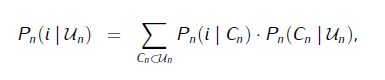
\includegraphics[width=0.5\textwidth, angle=0]{understanding/figures/dc.png} \end{center}

% ##################################################################################################################
This chapter (i) attempts to reconcile MATSim's mechanisms of plan
{}``mutation'', {}``selection'' and {}``execution'', borrowed from evolutionary computation, with a 
%mainstream
discrete choice perspective, and (ii) and sketches a solution to the
plan choice set generation problem.

Let $\mathcal{U}_n$ be the universal set of all plans that may ever be considered
by agent $n$, and denote by $C_{n}$ the concrete plan choice set
of that agent. The choice set independent probability that agent $n$
selects plan $i$ for execution can then be written as
\begin{eqnarray}
P_{n}(i\mid \mathcal{U}_n) & = & \sum_{C_{n}\subset \mathcal{U}_n}P_{n}(i\mid C_{n})\cdot P_{n}(C_{n}\mid \mathcal{U}_n),
\label{eq:unconditional-choice-proba}
\end{eqnarray}
which means the following. Selecting a plan requires a plan choice
set. The term $P_{n}(C_{n}\mid \mathcal{U}_n)$ represents the probability that
this concrete choice set is $C_{n}$, which must be a subset of $\mathcal{U}_n$.
Technically, the plan innovation modules draw from this distribution.
The term $P_{n}(i\mid C_{n})$ represents the probability that agent
$n$ selects plan $i$ given that its concrete choice set is $C_{n}$.
Technically, the plan selection modules draw from this distribution.
The product of these terms hence represents the probability that both
the choice set $C_{n}$ is available and that plan $i$ is chosen out
of that set. The probability of selecting plan $i$ independently
of the concrete choice set then results from adding the probabilities
of selecting it in the presence of all possible choice sets $C_{n}\subset \mathcal{U}_n$.

One observes in \MyEqRef{eq:unconditional-choice-proba} that the
behavior of an agent depends on both the choice model and the way
in which the choice set is generated, both of which are addressed
in the following.

% ##################################################################################################################
\section{\label{sec:Evaluating-choice-models}Evaluating choice models in
a simulated environment}

The discussion provided in this section focuses on the choice distribution
$P_{n}(i\mid C_{n})$ for given choice sets. In MATSim, a plan is
evaluated in terms of its score, and plan selection is based on the
score as the sole property of the plan. This is only a technical specification;
the scoring and selection protocols are responsible of representing
adequate perceptional and behavioral mechanisms. The notions of {}``choice''
and {}``selection'' are subsequently used interchangeably. \note{Parts of this had been suggested in an earlier Email. Not sure where else it may show up.}

The usual selection protocol of MATSim resembles a multinomial logit
choice model. Letting $S_{ni}$ be the score of plan $i$ of agent
$n$, one has
\begin{eqnarray}
P_{n}(i\mid C_{n}) & = & \frac{e^{\mu S_{ni}}}{\sum_{j\in C_{n}}e^{\mu S_{nj}}}\label{eq:ExpBetaPlanSelector}
\end{eqnarray}
with $\mu$ controlling the preference for higher scores.
It is set to one in the remainder of this section. Only if the score
of a plan represented its expected utility, then this would constitute
a plain multinomial logit choice model with $\mu$ taking the role
of a scale parameter. However, things are somewhat more complicated.

Assume that the attribute vector $\mathbf{x}_{ni}$ of the alternatives in \MyEqRef{eq:ExpBetaPlanSelector}
is defined through (a transformation of) the network conditions observed
during the last iteration(s). Assume further that the score is a linear
function of these attributes:
\begin{eqnarray}
S_{ni} & = & \boldsymbol{\beta}^{T}\mathbf{x}_{ni}\\
 & = & \boldsymbol{\beta}^{T}(\text{E}\{\mathbf{x}_{ni}\}+\boldsymbol{\eta}_{ni})\label{eq:score}
\end{eqnarray}
where $\boldsymbol{\beta}$ is a coefficient vector, superscript $T$ denotes the transpose,
and $\boldsymbol{\eta}_{ni}$ is a zero mean random vector. 
In the general case of $S_{ni}$ being a random
variable and not just an expected value, one obtains a mixture-of-logit
model with the choice distribution
\begin{eqnarray}
P_{n}(i\mid C_{n}) & = & 
\int\frac{\exp\left(\boldsymbol{\beta}^{T}\text{E}\{\mathbf{x}_{ni}\}+\boldsymbol{\beta}^{T}\boldsymbol{\eta}_{ni}\right)}
{\sum_{j\in C_{n}}\exp\left(\boldsymbol{\beta}^{T}\text{E}\{\mathbf{x}_{nj}\}+\boldsymbol{\beta}^{T}\boldsymbol{\eta}_{nj}\right)}
p(\boldsymbol{\eta}_{n})d\boldsymbol{\eta}_{n}\label{eq:mixture-of-logit}
\end{eqnarray}
where $p(\boldsymbol{\eta}_{n})$ is the probability density function of 
$\boldsymbol{\eta}_{n}=(\boldsymbol{\eta}_{ni})$, i.e. the joint probability
density function of the random disturbances of all alternatives of individual $n$.
\citep{train-2003}. This formulation comprises most if not all MATSim
configurations currently used. It represents the \lstinline{ExpBetaPlanSelector}
and the equivalent \lstinline{ExpBetaPlanChanger}. It also comprises
the \lstinline{BestPlanSelector} because that is equivalent to the \lstinline{ExpBetaPlanSelector}
with a very large (infinite) $\mu$. Arbitrary score averaging schemes
are also included; this only leads to different instances of $p(\boldsymbol{\eta}_{n})$.

Mainstream applications of mixture-of-logit models attempt to combine
the tractability of closed-form logit models with the flexibility of
simulating arbitrary $p(\boldsymbol{\eta}_n)$ distributions.
The distribution of $\boldsymbol{\eta}_n$ is often as simple as a multivariate normal
because this already allows to introduce rich correlation structures
into the underlying random utilities. In MATSim, however, the simulated
error term $\boldsymbol{\eta}_n$ is extremely complicated. Revisiting \MyEqRef{eq:score},
it defines the variability of the score that results from the fact
that the simulated network conditions are stochastic. The distribution
from which these network conditions are drawn is defined implicitly
through the mobility simulation. It is not available in closed form;
one can only draw from it.

Additional complexity results from the simulated network conditions
being in turn the consequence of simulated travel behavior that is
again defined through \MyEqRef{eq:mixture-of-logit}. This circular
dependency is natural, given that MATSim is mainly a transport planning
model, (see Chapter~\ref{ch:montecarlo}). Indeed, just as a representation
of the mutual demand/supply dependency is essential in transport planning,
the circular definition of the $\boldsymbol{\eta}_n$ terms adds realism to MATSim:
\begin{enumerate}
\item Assume one could somehow make the simulated network conditions more
realistic. The result would be a more realistic distribution $p(\boldsymbol{\eta}_n)$
of the simulated error terms.
\item All else equal, increasing the realism of $p(\boldsymbol{\eta}_n)$ in \MyEqRef{eq:mixture-of-logit}
would also increase the realism of the resulting choice distributions.
\item This in turn would lead to the selection of more realistic travel
plans, with the consequence that their execution would result in even
more realistic network conditions.
\end{enumerate}
However, this positive feedback only applies to the extent to which
the random error terms of the postulated behavioral model are indeed
outputs of the mobility simulation. Simulated travel time (variability)
is such a case. Unobserved preferences of the decision maker, however,
are not an output of the mobility simulation and hence need to be
captured otherwise. (The extreme case of a choice distribution that
results from combining a stochastic mobility simulation with a best-response
plan selection hence constitutes only a limited, so to say {}``mechanical''
perspective on travel behavior.)

How to insert the randomness of the simulated network conditions into
$\boldsymbol{\eta}_n$ is a delicate problem. The notion of {}``learning'' again
enters the picture, and again it is not particularly helpful, cf.
Chapter~\ref{ch:montecarlo}: If the simulation iterations really represented
simulated days, a model of real human learning would be needed in
order to combine a sequence of past network conditions into an instantaneous
$\boldsymbol{\eta}_n$ realization. Without a sound instance of such a learning model,
a behavioral justification of \MyEqRef{eq:mixture-of-logit} cannot
be given.

However, another perspective on this problem is possible, continuing
the arguments of Chapter~\ref{ch:montecarlo}. It is argued there that
the sole purpose of MATSim's iterative mechanism is to attain a realistic
stationary distribution. If so, then the sole purpose of the simulated
$\boldsymbol{\eta}_n$s is to yield a realistic stationary choice distribution. To
illustrate this perspective, consider the following moving-average score
updating rule:
\begin{eqnarray}
\bar{S}_{ni}^{k+1} & = & \begin{cases}
\alpha S_{ni}^{k} + (1 - \alpha)\bar{S}_{ni}^{k} & \text{if }n\text{ chose plan }i\\
\bar{S}_{ni}^{k} & \text{otherwise}
\end{cases}
\end{eqnarray}
where $\bar{S}^{k}$ is the filtered score of iteration $k$ and $S^{k}$
is the concrete score observed in that iteration. The learning rate $\alpha$
controls how strongly the filtered score is smoothed out, and hence
it controls the variability of $\boldsymbol{\eta}_n$. MATSim enables this mechanism
through the \lstinline{learningRate} parameter.

Assuming for simplicity that upon convergence the unfiltered stationary score
$S_{ni}^{\infty}$ fluctuates independently from iteration to
iteration around its expected value, one can derive the following 
(as demonstrated in the appendix to this chapter):
\begin{eqnarray}
\text{E}\{\bar{S}_{ni}^{\infty}\} & = & \text{E}\{S_{ni}^{\infty}\}\\
\text{VAR}\{\bar{S}_{ni}^{\infty}\} & = & \frac{\alpha}{2-\alpha}\text{VAR}\{S_{ni}^{\infty}\}.
\end{eqnarray}
$\bar{S}$ is unbiased with respect to the underlying score process
and its variance is in the interval from zero to $\text{VAR}\{S\}$,
depending on the chosen $\alpha$. There is no need to justify this
through a learning process. One merely has constructed a parametrization
of the distribution $p(\boldsymbol{\eta}_n)$. In the resulting
mixture model \MyEqRef{eq:mixture-of-logit}, $\alpha$ should be
estimated from real data, just as any other parameter of that model.


% ##################################################################################################################
\section{\label{sec:Evolution-of-choice}Evolution of choice sets in a simulated
environment}

This section turns to the question what it means to insert a plan
innovation mechanism into MATSim's iterated simulation logic. The
modeling of a choice set is, even in the discrete choice community,
quite controversial \citep{frejinger-2010}, and there is no reason
to believe that {}``plan mutation'' or {}``plan innovation'' in
MATSim are more realistic than anything proposed in that community.
However, as said before, if the choice sets are {}``wrong'' (whatever
this may precisely mean) then one can be fairly confident that the
simulated behavior also turns out wrong.
%\kai{gunnar, pls chk following paragraph.} To illustrate that last statement:
%
For example, if all alternatives in the synthetic choice set are very different from the alternative that is used in the real world, it is quite improbable that the simulation will display correct aggregated quantities, and it is even more improbable that the simulation will have useful sensitivities to policy measures.

%%\kai{Ich würde das so nicht unterschreiben.  Irgendwie brauchen wir aber einen Weg, wie wir das in diesem Buch zur Konvergenz bringen.  EINE Möglichkeit wäre, dass wir an mehreren Stellen so etwas wie ``Also see Sec.??? for a discussion.'', und versuchen dann, dort auf Formulierungen zu kommen, auf die wir uns einigen können.  Das wäre dann ``research avenues'', was es dann logischerweise ist.}

%%\kai{Inhaltlich: Wenn ich mir so etwas wie das Buch von Norvig/Russel anschaue, dann kann man m.E.\ nicht behaupten, dass im Umfeld von ``artificial intelligence'' (AI) nichts passiert ist.   Mein Eindruck ist eher, dass Fortschritt vor allem dann passiert, wenn die ``intuitiveren'' Methoden aus AI sich mit den ökonometrischen Methoden irgendwie einigen.  Deshalb will ich auch keine Gegnerschaft zwischen ``MATSim'' und sogenannten ``more mainstream methods''.  Selbst wenn Dinge wie ``genetic algorithms'', ``simulated annealing'', ``neuronale Netze'' bereits bekannte statistische Methoden neu erfinden, so ist es dennoch so, dass sie vielleicht ein gutes ``Bild'' finden, was die Methode viel zugänglicher macht.  Und schlussendlich wollen wir mit MATSim kein perfektes ökonometrisches Modell, sondern etwas, was in der Praxis gut funktioniert.  Und bisher hat es tatsächlich recht gut funktioniert, das choice set einfach heuristisch zusammenzusetzen, und dann mit starker Betonung der guten Lösungen auszuwählen.  Es spricht nichts dagegen, zu \emph{untersuchen}, ob man es besser machen kann.  Aber ohne  klaren Nachweis, dass man mit einer stärker ökonometrischen Methode wirklich für die Praxis brauchbarer wird, möchte ich die (für Nicht-Ökonometriker) besser verständliche Variante gerne auch behalten.  --  Der deutsche BVWP macht übrigens Routenwahl \emph{nur} basierend auf ``fastest route'', und hat noch nicht einmal ein konvergierendes Verfahren.}

MATSim performs in every iteration the following operations for each
agent: (1) update of the choice set and (2) choice of a plan from
the updated choice set, using the model (\ref{eq:ExpBetaPlanSelector}).
To make the simulated long-term (stationary) plan choice independent
of the plan choice set generation, one may require the following stationary
choice distribution:
\begin{eqnarray}
P_{n}(i\mid \mathcal{U}_n) & = & \frac{e^{\mu S_{ni}}}{\sum_{j\in \mathcal{U}_n}e^{\mu S_{nj}}},
\label{eq:global-choice-model}
\end{eqnarray}
meaning that plans are selected from the universal choice set.

Denoting further by $P(C_{n}\rightarrow C_{n}')$ the probability
that plan mutation/innovation turns the choice set $C_{n}$ into $C_{n}'$,
it is possible to enforce the long-term choice distribution \MyEqRef{eq:global-choice-model}
through an application of the Metropolis-Hastings (MH) algorithm \citep{hastings-1970}.
(See also \citet{floetteroed-2012b} for a related approach to a similar
problem.) 

The MH algorithm specifies the transition distribution
of a Markov chain such that a desired stationary distribution of that
chain is reached. Given that Chapter~\ref{ch:montecarlo} has established
a formulation of MATSim in terms of such a chain, the MH machinery can
hence be inserted into the MATSim iterations. A simplification made in
the following is that the choice distribution of agent $n$ is considered
independent of all other agents.

To make this concrete, the state space of the algorithm is defined as the tuple
$(C_{n},\, i\in C_{n})$ consisting of choice set and resulting choice.
During each (MATSim) iteration, one first draws a new choice set $C_{n}'$,
then draws a new choice $i'\in C_{n}'$, and finally accepts the new
state $(C_{n}',\, i')$ with probability
\begin{eqnarray}
\phi[(C_{n},\, i),(C_{n}',\, i')] 
& = & 
\min\left\{ 
\frac{{\displaystyle P_{n}(i'\mid \mathcal{U}_n)}}
{{\displaystyle P_{n}(i\mid \mathcal{U}_n)}}
\cdot
\frac{{P(C_{n}'\rightarrow C_{n})P_n(i\mid C_{n})}}
{{P(C_{n}\rightarrow C_{n}')P_n(i'\mid C_{n}')}}
,\,1\right\} 
\label{eq:accept-proba-1}
\end{eqnarray}
and rejects it otherwise (meaning that the original choice set $C_{n}$
and choice $i\in C_{n}$ are maintained).
Technically, the first fraction introduces a preference for states
that comprise a more probable choice, and the second
fraction corrects for the way in which transitions between states are
proposed.

% \kai{Kann es sein, dass da der $n$-Index verrutscht ist:
% \begin{eqnarray}
% \phi & = & \min\left\{ \frac{{\displaystyle P_{n}(i'\mid C)P(C_{n}'\rightarrow C_{n})P_n(i\mid C_{n})}}{{\displaystyle P_{n}(i\mid C)P(C_{n}\rightarrow C_{n}')P_n(i'\mid C_{n}')}},\,1\right\} \label{eq:accept-proba-1}
% \end{eqnarray}
% ?? --  Ich finde das mit dem $C$ ohne $n$-Index schwer zu lesen; vielleicht doch $\tilde C_n$?}

Assume that the plan innovation yields exactly
one new plan $i_{\text{in}}$ through a best-response against the
last iteration. The corresponding plan innovation distribution is
approximated by $e^{\mu_{\text{inno}}S_{ni}}/\sum_{j\in \mathcal{U}_n}e^{\mu_{\text{inno}}S_{nj}}$,
with a very large $\mu_{\text{inno}}$. Assuming further that $i_{\text{in}}$
replaces exactly one uniformly selected plan $i_{\text{out}}$, 
which implies that the choice set size $J$ is constant, 
and excluding for simplicity the case that the best response innovation
reconstructs exactly the removed plan,
one obtains
\begin{eqnarray}
P(C_{n}\rightarrow C_{n}') & = & \frac{1}{J}\cdot\frac{e^{\mu_{\text{inno}}S_{ni_{\text{in}}}}}{\sum_{j\in \mathcal{U}_n}e^{\mu_{\text{inno}}S_{nj}}}\\
P(C_{n}'\rightarrow C_{n}) & = & \frac{1}{J}\cdot\frac{e^{\mu_{\text{inno}}S_{ni_{\text{out}}}}}{\sum_{j\in \mathcal{U}_n}e^{\mu_{\text{inno}}S_{nj}}}.
\end{eqnarray}
Inserting this as well as \MyEqRef{eq:ExpBetaPlanSelector} and \MyEqRef{eq:global-choice-model}
into \MyEqRef{eq:accept-proba-1}, one obtains
\begin{eqnarray}
\phi[(C_{n},\, i),(C_{n}',\, i')] & = & 
\min\left\{ 
\frac{e^{\mu S_{ni'}}}{e^{\mu S_{ni}}}\cdot
\frac{{\displaystyle e^{\mu_{\text{inno}}S_{ni_{\text{out}}}}\frac{\displaystyle e^{\mu S_{ni}}}{\sum_{j\in C_{n}}\displaystyle e^{\mu S_{nj}}}}}
{{\displaystyle e^{\mu_{\text{inno}}S_{ni_{\text{in}}}}\frac{\displaystyle e^{\mu S_{ni'}}}{\sum_{j\in C_{n}'} \displaystyle e^{\mu S_{nj}}}}},\,1\right\} \\
 & = & 
 \min\left\{ 
 {\displaystyle e^{\mu_{\text{inno}}(S_{ni_{\text{out}}}-S_{ni_{\text{in}}})}} \cdot
 \frac{\sum_{j\in C_{n}'} \displaystyle e^{\mu S_{nj}}}{\sum_{j\in C_{n}} \displaystyle e^{\mu S_{nj}}},\,1\right\} 
\end{eqnarray}
and hence
\begin{eqnarray}
\lim_{\mu_{\text{inno}}\rightarrow\infty}
\phi[(C_{n},\, i),(C_{n}',\, i')] & = & \text{Pr}(S_{ni_{\text{out}}}\geq S_{ni_{\text{in}}}).
\end{eqnarray}
Some care is needed when evaluating this expression because it assumes
$S_{ni_{\text{in}}}$ and $S_{ni_{\text{out}}}$ to be independent
random variables, whereas $S_{ni_{\text{in}}}$ is (due to the best
response) always maximal among all alternatives given the most recent
iteration. One should hence evaluate this expression by computing
both scores from the network conditions of two randomly selected stationary
iterations.

This allows to select plans according to (\ref{eq:global-choice-model})
from an unconstrained choice set even though one enumerates only a
small subset of the full choice set, which is updated through a computationally
efficient best-response mechanism. In summary, one does the following
for each agent in each iteration:
\begin{compactenum}
\item Randomly select a given plan for removal and compute a new best response
plan against the last iteration.
\item Is, based on network conditions from two randomly selected stationary
iterations, the new plan better than the one selected for removal?

\begin{compactitem}
\item Yes: Keep the previously selected plan and the previous choice set.
\item No: Remove the randomly selected plan from the choice set, add the
newly generated plan, and select a new plan from the new choice set.
\end{compactitem}
\end{compactenum}
This at first glance counter-intuitive behavior can be motivated as follows:
%\kai{previous sentence changed; pls check} 
Best response creates new plans that are by chance
better than any other plan in a given iteration. Best response is
hence corrected for by accepting the new plan only if it is by chance
worse than a randomly selected alternative plan, with both plans being
evaluated in randomly selected stationary iterations.

Note that the correctness of this approach depends on the ability
of the best-response plan innovation to create plans that are sufficiently
variable, in the sense that the plan choice set innovation process
is irreducible \citep{ross-2006}.

% ##################################################################################################################
\section{\label{sec:Summary}Summary}
This chapter attempted to phrase MATSim's mechanisms of plan scoring,
innovation, mutation and selection in the somewhat more mainstream
terminology of discrete choice modeling. The implications of evaluating
stochastic scores when selecting a plan were explained. Further, a
cure to the possibly detrimental effect of using best-response plan
innovation modules was suggested.

% ##################################################################################################################

\section*{Appendix: Derivation of filtered score statistics}

Writing out the expectation:
\begin{eqnarray}
\text{E}\{\bar{S}_{ni}^{k+1}\} & = & P_{n}(i)\text{E}\{\alpha S_{ni}^{k}+(1-\alpha)\bar{S}_{ni}^{k}\}+(1-P_{n}(i))\text{E}\{\bar{S}_{ni}^{k}\}\\
% & = & \alpha P_{n}(i)\text{E}\{S_{ni}^{k}\}+P_{n}(i)\text{E}\{\bar{S}_{ni}^{k}\}-\alpha P_{n}(i)\text{E}\{\bar{S}_{ni}^{k}\}+\text{E}\{\bar{S}_{ni}^{k}\}-P_{n}(i)\text{E}\{\bar{S}_{ni}^{k}\}\\
\Leftrightarrow\text{E}\{\bar{S}_{ni}^{k+1}\}-\text{E}\{\bar{S}_{ni}^{k}\} & = & \alpha P_{n}(i)(\text{E}\{S_{ni}^{k}\}-\text{E}\{\bar{S}_{ni}^{k}\}).
\end{eqnarray}
From $\lim_{k\rightarrow\infty}\text{E}\{\bar{S}_{ni}^{k+1}\}-\text{E}\{\bar{S}_{ni}^{k}\}=0$
then follows
\begin{eqnarray}
\lim_{k\rightarrow\infty}\left(\text{E}\{S_{ni}^{k}\}-\text{E}\{\bar{S}_{ni}^{k}\}\right) & = & 0. \label{eq:first-score-moment}
\end{eqnarray}
%
Proceeding similarly for the second moment:
\begin{eqnarray}
\text{E}\{(\bar{S}_{ni}^{k+1})^{2}\} 
& = & 
P_{n}(i)\text{E}\{(\alpha S_{ni}^{k}+(1-\alpha)\bar{S}_{ni}^{k})^{2}\}+(1-P_{n}(i))\text{E}\{(\bar{S}_{ni}^{k})^{2}\}\\
%& = & 
%P_{n}(i)\text{E}\{\alpha^{2}(S_{ni}^{k})^{2}+2\alpha(1-\alpha)S_{ni}^{k}\bar{S}_{ni}^{k}+(1-\alpha)^{2}(\bar{S}_{ni}^{k})^{2}\}+(1-P_{n}(i))\text{E}\{(\bar{S}_{ni}^{k})^{2}\}\\
%& = & 
%\alpha^{2}P_{n}(i)\text{E}\{(S_{ni}^{k})^{2}\}+2\alpha(1-\alpha)P_{n}(i)\text{E}\{S_{ni}^{k}\}^{2}+(1-\alpha)^{2}P_{n}(i)\text{E}\{(\bar{S}_{ni}^{k})^{2}\}+(1-P_{n}(i))\text{E}\{(\bar{S}_{ni}^{k})^{2}\}\\
\Leftrightarrow
\text{E}\{(\bar{S}_{ni}^{k+1})^{2}\}-\text{E}\{(\bar{S}_{ni}^{k})^{2}\} 
%& = & \alpha^{2}P_{n}(i)\text{E}\{(S_{ni}^{k})^{2}\}+2\alpha(1-\alpha)P_{n}(i)\text{E}\{S_{ni}^{k}\}^{2}+(1-2\alpha+\alpha^{2})P_{n}(i)\text{E}\{(\bar{S}_{ni}^{k})^{2}\}-P_{n}(i)\text{E}\{(\bar{S}_{ni}^{k})^{2}\}\\
%& = & \alpha^{2}P_{n}(i)\text{E}\{(S_{ni}^{k})^{2}\}+2\alpha(1-\alpha)P_{n}(i)\text{E}\{S_{ni}^{k}\}^{2}+(-2\alpha+\alpha^{2})P_{n}(i)\text{E}\{(\bar{S}_{ni}^{k})^{2}\}\\
& = & P_{n}(i) \alpha \left[\alpha\text{E}\{(S_{ni}^{k})^{2}\}+2(1-\alpha)\text{E}\{S_{ni}^{k}\}^{2}-(2-\alpha)\text{E}\{(\bar{S}_{ni}^{k})^{2}\}\right]
\end{eqnarray}
From $\lim_{k\rightarrow\infty}\text{E}\{(\bar{S}_{ni}^{k+1})^{2}\}-\text{E}\{(\bar{S}_{ni}^{k})^{2}\}=0$
then follows
\begin{eqnarray}
%\text{lim}_{k\rightarrow\infty}\alpha(2-\alpha)P_{n}(i)\text{E}\{(\bar{S}_{ni}^{k})^{2}\} 
%& = & 
%\text{lim}_{k\rightarrow\infty}\left[\alpha^{2}P_{n}(i)\text{E}\{(S_{ni}^{k})^{2}\}-2\alpha(1-\alpha)P_{n}(i)\text{E}\{S_{ni}^{k}\}^{2}\right]\\
\text{lim}_{k\rightarrow\infty}\text{E}\{(\bar{S}_{ni}^{k})^{2}\} 
%& = & \frac{\alpha^{2}}{\alpha(2-\alpha)}\text{E}\{(S_{ni}^{k})^{2}\}-\frac{2\alpha(1-\alpha)}{\alpha(2-\alpha)}\text{E}\{S_{ni}^{k}\}^{2}\\
& = & 
\frac{\alpha}{2-\alpha}\text{E}\{(S_{ni}^{k})^{2}\}-\frac{2-2\alpha}{2-\alpha}\text{E}\{S_{ni}^{k}\}^{2}. \label{eq:second-score-moment}
\end{eqnarray}
%
The limiting variance then results from inserting of \MyEqRef{eq:first-score-moment} and \MyEqRef{eq:second-score-moment} into
\begin{eqnarray}
\text{lim}_{k\rightarrow\infty}\text{VAR}\{\bar{S}_{ni}^{k}\} 
& = & \text{lim}_{k\rightarrow\infty}\left[\text{E}\{(\bar{S}_{ni}^{k})^{2}\}-\text{E}\{\bar{S}_{ni}^{k}\}^{2}\right]\\
% & = & \frac{\alpha}{2-\alpha}\text{E}\{(S_{ni}^{k})^{2}\}-\frac{2-2\alpha}{2-\alpha}\text{E}\{S_{ni}^{k}\}^{2}-\frac{2-\alpha}{2-\alpha}\text{E}\{S_{ni}^{k}\}^{2}\\
% & = & \frac{\alpha}{2-\alpha}\text{E}\{(S_{ni}^{k})^{2}\}+\frac{\alpha}{2-\alpha}\text{E}\{S_{ni}^{k}\}^{2}\\
 & = & \frac{\alpha}{2-\alpha}\text{VAR}\{(S_{ni}^{k})^{2}\}.
\end{eqnarray}
